
\documentclass[12pt, a4paper]{report}
\usepackage{epsfig}
\usepackage{subfigure}
%\usepackage{amscd}
\usepackage{amssymb}
\usepackage{graphicx}
%\usepackage{amscd}
\usepackage{amssymb}
\usepackage{subfiles}
\usepackage{framed}
\usepackage{subfiles}
\usepackage{amsthm, amsmath}
\usepackage{amsbsy}
\usepackage{framed}
\usepackage[usenames]{color}
\usepackage{listings}
\lstset{% general command to set parameter(s)
	basicstyle=\small, % print whole listing small
	keywordstyle=\color{red}\itshape,
	% underlined bold black keywords
	commentstyle=\color{blue}, % white comments
	stringstyle=\ttfamily, % typewriter type for strings
	showstringspaces=false,
	numbers=left, numberstyle=\tiny, stepnumber=1, numbersep=5pt, %
	frame=shadowbox,
	rulesepcolor=\color{black},
	,columns=fullflexible
} %
%\usepackage[dvips]{graphicx}
\usepackage{natbib}
\bibliographystyle{chicago}
\usepackage{vmargin}
% left top textwidth textheight headheight
% headsep footheight footskip
\setmargins{3.0cm}{2.5cm}{15.5 cm}{22cm}{0.5cm}{0cm}{1cm}{1cm}
\renewcommand{\baselinestretch}{1.5}
\pagenumbering{arabic}
\theoremstyle{plain}
\newtheorem{theorem}{Theorem}[section]
\newtheorem{corollary}[theorem]{Corollary}
\newtheorem{ill}[theorem]{Example}
\newtheorem{lemma}[theorem]{Lemma}
\newtheorem{proposition}[theorem]{Proposition}
\newtheorem{conjecture}[theorem]{Conjecture}
\newtheorem{axiom}{Axiom}
\theoremstyle{definition}
\newtheorem{definition}{Definition}[section]
\newtheorem{notation}{Notation}
\theoremstyle{remark}
\newtheorem{remark}{Remark}[section]
\newtheorem{example}{Example}[section]
\renewcommand{\thenotation}{}
\renewcommand{\thetable}{\thesection.\arabic{table}}
\renewcommand{\thefigure}{\thesection.\arabic{figure}}
\title{Research notes: linear mixed effects models}
\author{ } \date{ }


\begin{document}
	\author{Kevin O'Brien}
	\title{Mixed Models for Method Comparison Studies}
	\tableofcontents
	
\chapter{Appendices}
\section{Appendix 1 : Improper Method Comparison Techniques}
	The issue of whether two measurement methods are comparable to the extent that they can be used interchangeably with sufficient accuracy is encountered frequently in scientific research. Historically, comparison of two methods of measurement was carried
	out by use of paired sample $t-$test, 
	simple linear regression, or correlation coefficients. 
	
	
	\subsection*{Paired sample \emph{t-}test}
	\citet{Bartko} discusses the use of the well known paired sample $t$ test to test for inter-method bias; $H: \mu_{d}=0$. The test
	statistic is distributed as a $t$ random variable with $n-1$ degrees of freedom and is calculated as follows,
	\begin{equation}
	t^{*} = \frac{\bar{d}}{ s_d/\sqrt{n}}
	\end{equation}
	where $\bar{d}$ and $s_{d}$ is the average of the differences of the $n$ observations. This method can be potentially misused for method comparison studies. Paired $t-$tests test only whether the mean responses are the same, and so provides a useful test for inter-method bias. However, no insight can be obtained about the variability of the case-wise differences by the paired $t-$test, critically undermining it as a stand-alone procedure. Only if the two methods show comparable
	precision then the paired sample student $t$-test is appropriate for assessing the magnitude of the bias.
	
	%======================================================================================= %
	
	
	\subsection*{The Correlation Coefficient}
	%----------------------------------------------------------------------------%
	%		\subsection{Pearson's Correlation Coefficient} 
	% %- 			% http://www.jerrydallal.com/LHSP/compare.htm
	
	Correlation is inadequate to assess agreement because it only evaluates only the linear association of two sets of observations.  Nonetheless linear association is not the same as agreement. It is possible for two methods to
	be highly correlated, yet have poor agreement due to any combination of constant and proportional bias. Arguments against its usage have been made repeatedly in the relevant literature,  with \citet{BA83}, \citet{BA86}, \citet{BA2003} and \citet{giavarina2015understanding} as examples.
	%	
	%	
	%		
	%	
	%	The correlation coefficient can be close to 1 even when there is considerable bias between the two methods. For example, if one method gives measurements that are always 10 units higher than the other method, the correlation will be 1 exactly, but the measurements will always be 10 units apart.
	%	
	%	The magnitude of the correlation coefficient is affected by the range of subjects/units studied. 
	%	
	%	The correlation coefficient can be made smaller by measuring samples that are similar to each other and larger by measuring samples that are very different from each other. 
	%	
	
	%----------------------------------------------------------------------------%
	\subsection*{Regression Methods}
	On account of the fact that one set of measurements are linearly related to another, one could surmise that simple linear Regression is the most suitable approach to analyzing comparisons. However simple linear regression  is considered by many authors to be wholly unsuitable for method comparison studies \citep{BA83,CornCoch,ludbrook97}. Simple linear regression is defined as such with the name `Model I regression' by \citet{CornCoch}, in contrast to `Model II regression' models, which shall be discussed later on.
	
	A key assumptions of simple linear regression is that the independent variable values are without random error. 	
	For method comparison studies, both sets of measurement must be assumed to be measured with imprecision and neither case can be taken to be a reference method. Arbitrarily
	selecting either method as the reference (i.e. the independent variable) will yield conflicting outcomes: a regression of $X$ on $Y$ would yield an entirely different model from fitting $Y$ on $X$.
	
	Further criticisms of linear regression exist.
	Firstly regression methods are uninformative about the variability of the differences. Secondly regression models are unduly influenced by outliers. Lastly, regression models can not be used to effectively analyze repeated measurements.	
	
\subsubsection*{The Identity Plot}
	\citet{BA83} states that regression analysis can offer useful insights, and recommending an `Identity Plot', a simple graphical approach that yields a cursory examination of how well the measurement methods agree. In the case of good agreement, the co-variates of the Identity plot accord closely with the $X=Y$ line. This plot is not useful for a thorough examination of the data. \citet{BritHypSoc} notes that data points will tend to cluster around the line of equality,
	obscuring interpretation. An identity plot shall complement demonstrations of commonly used approaches in the next chapter.
	
	
	\subsubsection*{Decomposition of Inter-Method Bias}
	Regression approaches are useful for a making a detailed examination of the biases across the range of measurements, allowing inter-method bias to be decomposed into constant bias and proportional bias. Regression methods can determine the presence of inter-method bias, and the levels of constant bias and proportional bias thereof \cite{ludbrook97,ludbrook02}. 
	
	Constant bias describes the case where one method gives values that are consistently different to the other across the whole range. Using a naive estimation of bias, such as the mean of differences, it may incorrectly indicate absence of bias, by yielding a mean difference close to zero. This would be caused by positive differences in the measurements at one end of the range of measurements being canceled out by negative differences at the other end of the scale. Proportional Bias exists when two methods agree on average, but exhibit differences over a range of measurements, i.e. the differences are proportional to the scale of the measurement.	A measurement method may be subject to any combination of fixed bias or proportional bias, or both \citep{ludbrook02}. 
	
	Constant or proportional bias using linear regression can be detected by an individual test on the intercept or the slope of the line regressed from the results of the two methods to be compared. If there is no constant bias, the intercept is equal to zero and, similarly, if there is no proportional bias, the slope is equal to one. Thus, carrying out hypothesis tests on these coefficients (where the null hypotheses are $\beta_0=0$ and $\beta_1=1$) allow us to test for the presence of both types of bias.
	
	
	If the basic assumptions underlying linear regression are not met, the regression equation, and consequently the estimations of bias are undermined. 
	%Outliers are a source of error in regression estimates.
	

\section{Appendix 2 : Variations of the Bland-Altman Plot} 
The limits of agreement methodology assumes a constant level of bias throughout the range of measurements. As \citet*{BA86} point out this may not be the case. 
Importantly \citet{BA99} makes the following point:
\begin{quote}These estimates are meaningful only if we can assume
	bias and variability are uniform throughout the range of
	measurement, assumptions which can be checked graphically.
	\end{quote}
	
	The importance of this statement is that, should the Bland Altman plot indicate that these assumptions are not met, then their
	entire methodology, as posited thus far, is inappropriate for use
	in a method comparison study. Again, in the context of potential
	outlier in the Grubbs data (figure 1.2), this raises the question
	on how to correctly continue. 
	
	Due to limitations of the conventional difference plot, a series of alternative formulations for the Bland-Altman approach have been proposed. Referring to the assumption that bias and variability are constant across the range of measurements, \citet{BA99} address the case where there is an increase in variability as the magnitude increases. They remark that it is possible to ignore the issue altogether, but the limits of agreement would be wider apart than necessary when just lower magnitude measurements are considered. Conversely the limits would be too narrow should only higher magnitude measurements be used. 
	
	To address the issue, they propose the logarithmic transformation of the data. The plot is then formulated as the difference of paired log values against their mean. Bland and Altman acknowledge that this is not easy to interpret, and may not be suitable in all cases.
	
	\citet{BA99} offers two variations of the Bland-Altman plot that are intended to overcome potential problems that the conventional plot would be inappropriate for. The first variation is a plot of case-wise differences as percentage of averages, and is appropriate when there is an increase in variability of the differences as the magnitude increases. 
	
	The second variation is a plot of case-wise ratios as percentage of averages, removing the need for logarithmic transformation. This approach is useful when there is an increase in variability of the differences as the magnitude of the measurement increases. \citet{Eksborg} proposed such a ratio plot, independently of Bland and Altman. \citet{Dewitte} commented on the reception of this article by saying `\textit{Strange to say, this report has been overlooked}'.
	
	%%%%%%%%%%%%%%%%%%%%%%%%%%%%%%%%%%%%%%%%%%%%%%%
  
  \section{Appendix 3 : The Coefficient of Repeatability}
  
  
  \citet{BA99} strongly recommends the simultaneous estimation of repeatability and agreement by  collecting replicated data. \citet{ARoy2009} notes the lack of convenience in such calculations. The coefficient of repeatability is a measure of how well a measurement method agrees with itself over replicate measurements \citep{BA99}. 
  
  As mentioned previously, \citet{Barnhart} emphasize the importance of repeatability as part of an overall method comparison study. The coefficient of repeatability was proposed by \citet{BA99}, and is referenced in subsequent papers, such as \citet{BXC2008}. \citet{BSIrepeat} define a coefficient of
  repeatability as \emph{the value below which the difference between two single test results....may be expected to lie within a specified probability.} \citet{BA99} defines the repeatability coefficient as the upper limits of a prediction interval for the absolute difference between two measurements by the same method on the same item under identical circumstances. % \citep{BXC2008}.	
  
  Once the within-item variability for both methods has been estimated, the relevant calculations for the coefficients of repeatability are straightforward.
  The coefficient is calculated from the within-item variability $\sigma^2_{m}$ as  $1.96 \times \sqrt{2} \times \sigma_m$ = $2.83 \sigma_m$. For $95\%$ of subjects, two replicated measurement by the same method will be within this repeatability coefficient.
  
  
  The coefficient of repeatability may provide the basis for the formulation a formal definition of a `gold standard'. For example, by determining the ratio of the repeatability coefficient $(CR)$ to the sample mean $\bar{X}$. Advisably the sample size should specified in advance. A gold standard may be defined as the method with the lowest value of $\lambda = CR /\bar{X}$ with $\lambda < 0.1\%$. Similarly, a silver standard may be defined as the method with the lowest value of $\lambda $ with $0.1\% \leq \lambda < 1\%$. Such thresholds are solely for expository purposes.
  
  %------------------------------------------------------------%
  %
  %
  %	
  %\section{Coefficient of Repeatability}
  %The Bland Altman method offers a measurement on the repeatability of the methods. The \emph{Coefficient of Repeatability} (CR) can be calculated as 1.96 (or 2) times the standard deviations of the differences between the two measurements ($d_2$ and $d_1$).		
  %
  %
  %%		
  %%If the standard deviation of a measurement is $\sigma$ the repeatability coefficient is $2\times\sqrt{2} \sigma = 2.83\times \sigma \approx 2.8 \sigma$.
  %%		$\sigma^2_{x}$ is the within-subject variance of method $x$. The repeatability coefficient is $2.77 \sigma_{x}$ (i.e. $1.96 \times \sqrt{2} \sigma_{x}$). 
  %		
  %		The repeatability of measurement methods is calculated
  %		differently under the two models  Under the model assuming
  %		exchangeable replicates (1), the repeatability is based only on
  %		the residual standard deviation, i.e. $2.8\sigma_m$
  %	
  %	
  %	 The coefficient is calculated from the residual standard deviation (i.e. $1.96 \times \sqrt{2} \times \sigma_m$ = $2.83 \sigma_m$).
  
  
  
  
  
  
  
  
  
  
  %The coefficient of repeatability is referenced in subsequent papers, such as \citet{BXC2008} and \citet{ARoy2009}. Furthermore this coefficient features in other branches of measurement analysis. 
  %\textbf{Find Some Papers to back this up}.
  
  %\section{Repeatability in Bland-Altman Blood Data Analysis}
  %
  %The Bland-Altman plot may also be used to assess a method's repeatability by comparing repeated measurements using one single measurement method on a sample of items.
  %
  %The plot can then also be used to check whether the variability or precision of a method is related to the size of the characteristic being measured.
  %
  %Since for the repeated measurements the same method is used, the mean difference should be zero.
  %Therefore the Coefficient of Repeatability (CR) can be calculated as 1.96 (often rounded to 2) times the standard deviation of the case-wise differences.
  %
  %
  % Two readings by the same method will be within $1.96
  %		\sqrt{2} \sigma_w $ or $2.77 \sigma_w $ for 95\% of subjects. This value is called the repeatability coefficient.
  %		
  %		For observer J using the sphygmomanometer $ \sigma_w = \sqrt{37.408} = 6.116$ and so the repeatability coefficient is
  %		$2:77 \times 6.116 = 16:95$ mmHg.
  %		
  %		 For the machine S,$ \sigma_w = \sqrt{83.141} = 9.118$ and the repeatability coefficient is $2:77 \times 9.118 = 25.27$ mmHg.
  
\subsection{Carstensen Coefficient of Repeatability}
	The limits of agreement are not always the only issue of interest, the assessment of method specific repeatability and reproducibility are of interest in their own right. Repeatability can only be assessed when replicate measurements by each method are available.
	
	Under the model for linked replicates, there are two possibilities depending on the circumstances. If the variation between replicates within item can be considered a part of the repeatability it will be $2.8 \sqrt{
		\omega^2 + \sigma^2_m}$.
	
	However, if replicates are taken under substantially
	different circumstances, the variance component $\omega^2$ may be considered irrelevant in the repeatability and one would therefore
	base the repeatability on the measurement errors alone, i.e. use $2.8 \sigma_m$.
	
	\section{Appendix 4 : Other Types of Studies}
	\citet{lewis} categorize method comparison studies into three	different types.  The key difference between the first two is
	whether or not a `gold standard' method is used. In situations where one instrument or method is known to be `accurate and
	precise', it is considered as the`gold standard' \citep{lewis}. A	method that is not considered to be a gold standard is referred to
	as an `approximate method'. In calibration studies they are	referred to a criterion methods and test methods respectively.
	
\smallskip \textbf{1. Calibration problems}. The purpose is to establish a
		relationship between methods, one of which is an approximate
		method, the other a gold standard. The results of the approximate
		method can be mapped to a known probability distribution of the
		results of the gold standard \citep{lewis1991}. In such studies, the gold standard method and corresponding approximate method are
		generally referred to a criterion method and test method
		respectively. \citet*{BA83} make clear that their framework is
		not intended for calibration problems.\\
		
\smallskip \textbf{2. Comparison problems}. When two approximate methods, that use the same units of measurement, are to be
			compared. This is the case which the Bland-Altman methodology is specfically intended for, and therefore it is the most relevant of
			the three.
			
\bigskip \textbf{3. Conversion problems}. When two approximate methods, that use different units of measurement, are to be
	compared. This situation would arise when the measurement methods	use 'different proxies', i.e different mechanisms of measurement.
	\citet{lewis} deals specifically with this issue. In the context of this study, it is the least relevant of the three.
	
\citet[p.47]{DunnSEME} cautions that`gold standards' should not be
	assumed to be error free. `It is of necessity a subjective decision when we come to decide that a particular method or
	instrument can be treated as if it was a gold standard'. The clinician gold standard, the sphygmomanometer, is used as an example thereof. The sphygmomanometer `leaves considerable room for improvement' \citep{DunnSEME}. \citet{pizzi} similarly addresses the issue of glod standards, `well-established gold standard may itself be imprecise or even unreliable'.
	
The NIST F1 Caesium fountain atomic clock is considered to be the gold standard when measuring time, and is the primary time and frequency standard for the United States. The NIST F1 is accurate	to within one second per 60 million years \citep{NIST}. In even extreme cases, there must be an assumption of inaccuracy with gold standard systems.

	
	Measurements of the interior of the human body are, by definition,
	invasive medical procedures. The design of method must balance the
	need for accuracy of measurement with the well-being of the
	patient. This will inevitably lead to the measurement error as
	described by \citet{DunnSEME}. The magnetic resonance angiogram,
	used to measure internal anatomy, is considered to the gold
	standard for measuring aortic dissection. Medical tests based upon
	the angiogram are reported to have a false positive reporting rate
	of 5\% and a false negative reporting rate of 8\% \citep{ACR}.
		

	In literature they are, perhaps more accurately, referred to as `fuzzy gold standards' \citep{phelps}. Consequently when one of the methods is
	essentially a fuzzy gold standard, as opposed to a `true' gold
	standard, the comparison of the criterion and test methods should
	be consider in the context of a comparison study, as well as of a
	calibration study.	
		

	
	
	\citet{Aroy2015} discusses the importance of gold standards in the context of method comparison studies.
	Currently the phrase `gold standard' describes the most accurate method of measurement available. No other criteria are set out. Further to \citet{DunnSEME}, various gold standards have a varying levels of repeatability. Dunn cites the example of the sphygmomanometer (i.e. a blood pressure measurement cuff), which is prone to measurement error. Consequently it can be said that a measurement method can be the `gold standard', yet have poor repeatability. \citet{DunnSEME} recognizes this problem. Hence, if the most accurate method is considered to have poor repeatability, it is referred to as a `bronze standard'.  Again, no formal definition of a bronze standard exists.
	
	% % % Bronze Standard
	
	
	\citet[p.47]{DunnSEME} cautions that `gold standards' should not be
	assumed to be error free and that `it is of necessity a subjective
	decision when we come to decide that a particular method or
	instrument can be treated as if it was a gold standard'. The
	clinician gold standard, the sphygmomanometer, is used as an
	example thereof.  The sphygmomanometer `leaves considerable room
	for improvement'. \citet{pizzi} similarly
	addresses the issue of gold standards, `well-established gold
	standard may itself be imprecise or even unreliable'.
	
	

	
	In literature gold standards are, perhaps more accurately, can be referred to as
	`fuzzy gold standards' \citep{phelps}. Consequently, when one of the methods is
	essentially a fuzzy gold standard, as opposed to a `true' gold standard, the comparison of the criterion and test methods should
	be consider both in the context of a comparison study and a	calibration study.
	
	
	According to Bland and Altman, one should use the approach previous outlined, even when one of the methods is a gold standard.
	
	
\subsection{Similar Problems}
\citet{lewis1991} categorize method comparison studies into three
different types, namely: calibration, comparison and conversion. The key difference between the first two is
whether or not a `gold standard' method is used. In situations
where one instrument or method is known to be `accurate and
precise', it is considered as the `gold standard' \citep{lewis1991}. A
method that is not considered to be a gold standard is referred to
as an `approximate method'. In calibration studies they are
referred to as criterion methods and test methods respectively.\\
\smallskip
\textbf{1. Calibration problems}. The purpose is to establish a
relationship between methods, one of which is an approximate
method, the other a gold standard. The results of the approximate
method can be mapped to a known probability distribution of the
results of the gold standard \citep{lewis1991}. In such studies, the
gold standard method and corresponding approximate method are
generally referred to a criterion method and test method respectively. \citet*{BA83} make clear that their framework is
not intended for calibration problems.\\
\smallskip \textbf{2. Comparison problems}. When two approximate methods, that use the same units of measurement, are to be
compared. This is the case for which Bland and Altman's Methodology is intended, and therefore it is the most relevant of
the three for this thesis.\\
\smallskip \textbf{3. Conversion problems}. When two approximate methods, that use different units of measurement, are to be	compared. This situation would arise when the measurement methods
use `different proxies', i.e different mechanisms of measurement.\\
\smallskip
\citet{lewis1991} deals specifically with this issue. In the context
of this thesis, it is the least relevant of the three cases.

\citet{Aroy2015} discusses the importance of gold Standards in the context of method comparison studies.
Currently the phrase `gold standard' describes the most accurate method of measurement available. No other criteria are set out. Further to \citet{DunnSEME}, various gold standards have a varying levels of repeatability. Dunn cites the example of the sphygmomanometer (i.e. a blood pressure measurement cuff), which is prone to measurement error. Consequently it can be said that a measurement method can be the `gold standard', yet have poor repeatability. \citet{DunnSEME} recognizes this problem. Hence, if the most accurate method is considered to have poor repeatability, it is referred to as a `bronze standard'.  Again, no formal definition of a bronze standard exists.

% % % Bronze Standard


\citet[p.47]{DunnSEME} cautions that `gold standards' should not be
assumed to be error free and that `it is of necessity a subjective
decision when we come to decide that a particular method or
instrument can be treated as if it was a gold standard'. The
clinician gold standard, the sphygmomanometer, is used as an
example thereof.  The sphygmomanometer `leaves considerable room
for improvement'. \citet{pizzi} similarly addresses the issue of gold standards, `well-established gold
standard may itself be imprecise or even unreliable'.


The NIST F1 Caesium fountain atomic clock is considered to be the gold standard when measuring time, and is the primary time and
frequency standard for the United States. The NIST F1 is accurate to within one second per 60 million years \citep{NIST}.

Measurements of the interior of the human body are, by definition,
invasive medical procedures. The design of method must balance the need for accuracy of measurement with the well-being of the	patient. This will inevitably lead to the measurement error as described by \citet{DunnSEME}. The magnetic resonance angiogram,
used to measure internal anatomy, is considered to the gold	standard for measuring aortic dissection. Medical tests based upon
the angiogram are reported to have a false positive reporting rate
of 5\% and a false negative reporting rate of 8\% \citep{ACR}.

In literature gold standards are, perhaps more accurately, can be referred to as
`fuzzy gold standards' \citep{phelps}. Consequently, when one of the methods is
essentially a fuzzy gold standard, as opposed to a `true' gold standard, the comparison of the criterion and test methods should
be consider both in the context of a comparison study and a	calibration study.




According to Bland and Altman, one should use the methodology
previous outlined, even when one of the methods is a gold standard.



\section{Appendix 5 : Indices and Graphical Techniques}

%%%%%%%%%%%%%%%%%%%%%%%%%%%%%%%%%%%%%%%%%%%%%%%%%%%%%%%%%%%%%%%%%%%%%%%%%

As an alternative to limits of agreement, \citet{lin2002} proposes the use of
the mean square deviation in assessing agreement. The mean square
deviation is defined as the expectation of the squared differences
of two readings. The MSD is usually used for the case of two
measurement methods $X$ and $Y$, each making one measurement for
the same subject, and is given by:
\[
MSDxy = E[(x - y)^2]  = (\mu_{x} - \mu_{y})^2 + (\sigma_{x} -
\sigma_{y})^2 + 2\sigma_{x}\sigma_{y}(1-\rho_{xy}).
\]


\citet{Barnhart} advises the use of a predetermined upper limit
for the MSD value, $MSD_{ul}$, to define satisfactory agreement.
However, a satisfactory upper limit may not be easily
determinable, thus creating a drawback to this technique.


Alternative indices, proposed by \citet{Barnhart}, are the square root of the MSD and the expected absolute difference (EAD). 
\[
EAD = E(|x - y|) = \frac{\sum |x_{i}- y_{i}|}{n},
\]
Both of these indices can be interpreted intuitively, since their units are the same as that of the original measurements. They can also be compared to the maximum acceptable absolute difference between two methods of measurement $d_{0}$. For the sake of brevity, the EAD will be considered solely.

The EAD can be used to supplement the inter-method bias in an
initial comparison study, as the EAD is informative as a measure
of dispersion, is easy to calculate and requires no distributional
assumptions. A consequence of using absolute differences is that high variances would result in a higher EAD value. 

% latex table generated in R 3.1.1 by xtable 1.7-4 package
% Mon Feb 23 21:12:33 2015
% latex table generated in R 3.1.1 by xtable 1.7-4 package
% Mon Feb 23 21:13:45 2015
% latex table generated in R 3.1.1 by xtable 1.7-4 package
% Mon Feb 23 22:10:26 2015
%\begin{table}[ht]
%	\centering
%	\begin{tabular}{r| rrrr}
%		\hline
%		\item & X & Y & U & V \\ 
%		\hline
%		1 & 101.83 & 102.52 & 98.05 & 99.53 \\ 
%		2 & 101.68 & 102.69 & 99.17 & 96.53 \\ 
%		3 & 97.89 & 99.01 & 100.31 & 97.55 \\ 
%		4 & 98.15 & 99.57 & 100.35 & 96.03 \\ 
%		5 & 99.94 & 100.85 & 99.51 & 99.00 \\ 
%		6 & 98.85 & 98.86 & 98.50 & 100.76 \\ 
%		7 & 99.86 & 97.85 & 100.66 & 99.37 \\ 
%		8 & 101.57 & 100.21 & 99.66 & 108.87 \\ 
%		9 & 100.12 & 99.85 & 99.70 & 105.16 \\ 
%		10 & 99.49 & 98.77 & 101.55 & 94.31 \\ 
%		\hline
%	\end{tabular}
%\end{table}




\begin{table}[ht]
	\centering
	\begin{tabular}{|c|c|c|c|c|}
		\hline
		& U & V & $U-V$ & $|U-V|$ \\ 
		\hline
		1 & 98.05 & 99.53 & -1.49 & 1.49 \\ 
		2 & 99.17 & 96.53 & 2.64 & 2.64 \\ 
		3 & 100.31 & 97.55 & 2.75 & 2.75 \\ 
		4 & 100.35 & 96.03 & 4.32 & 4.32 \\ 
		5 & 99.51 & 99.00 & 0.51 & 0.51 \\ 
		6 & 98.50 & 100.76 & -2.26 & 2.26 \\ 
		7 & 100.66 & 99.37 & 1.29 & 1.29 \\ 
		8 & 99.66 & 108.87 & -9.21 & 9.21 \\ 
		9 & 99.70 & 105.16 & -5.45 & 5.45 \\ 
		10 & 101.55 & 94.31 & 7.24 & 7.24 \\ 
		\hline
	\end{tabular}
	\caption{Example data set}
	\label{EADdata}
\end{table}

To illustrate the use of EAD, consider Table ~\ref{EADdata}. The inter-method bias of 0.03, which is desirably close to zero in the context of agreement. However, an identity plot would indicate very poor agreement, as the points are noticeably distant from the line of equality.
\begin{figure}
	\centering
	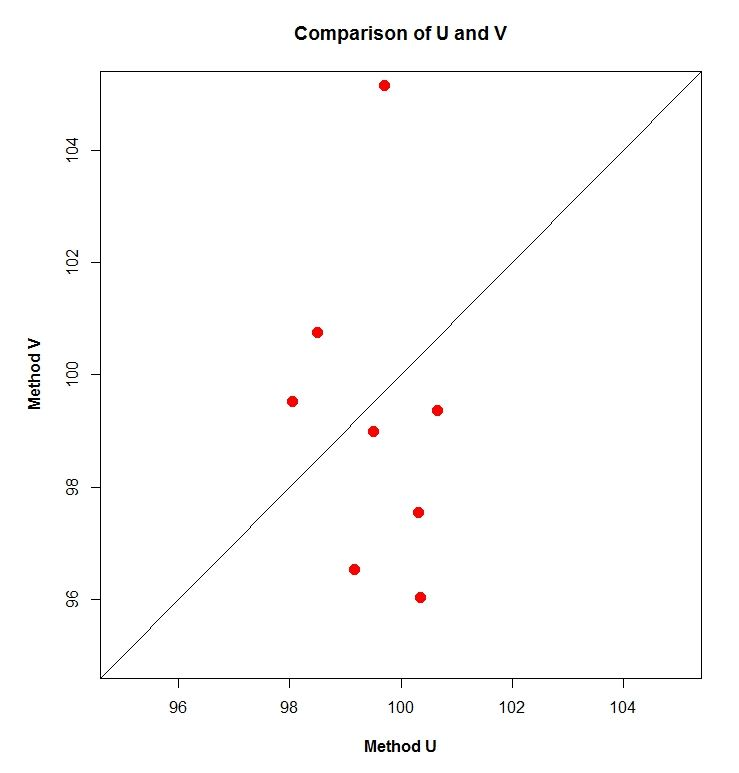
\includegraphics[width=0.5\linewidth]{EAD-UV}
	\caption{Identity Plot for example data}
	\label{fig:EADidentity}
\end{figure}

The limits of agreement are $[-9.61, 9.68]$, which is a wide interval for this data. As with the identity plot, this would indicate lack of agreement. As with inter-method bias, an EAD value close to zero is desirable. However, from Table ~\ref{EADdata}, the EAD can be computed as 3.71. The Bland-Altman plot remains a useful part of the analysis. In Figure \ref{fig:EAD1}, it is clear there is a systematic decrease in differences across the range of measurements.
\begin{figure}[h!]
	\centering
	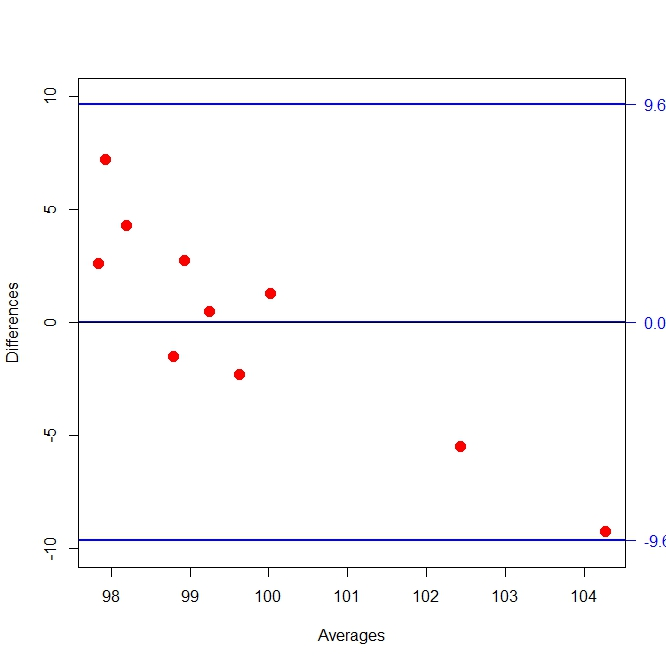
\includegraphics[width=0.55\linewidth]{images/EAD1}
	\caption{Bland-Altman Plot for UV comparison}
	\label{fig:EAD1}
\end{figure}

\citet{Barnhart} remarks that a comparison of EAD and MSD, using
simulation studies, would be interesting, while further adding
that `\textit{It will be of interest to investigate the benefits of these
	possible new unscaled agreement indices}'. For the Grubbs' `F vs C' and `F vs T' comparisons, the inter-method bias, difference variances, limits of agreement and EADs are shown
in Table 1.5. The corresponding Bland-Altman plots for `F vs C' and `F vs T' comparisons were depicted previously on Figure 1.3. While the inter-method bias for the `F vs T' comparison is smaller, the EAD penalizes the comparison for having a greater variance of differences. The EAD values for both comparisons are therefore much closer.
\begin{table}[ht]
	\begin{center}
		\begin{tabular}{|c||c|c|}
			\hline
			& F vs C & F vs T  \\\hline
			\hline
			Inter-method bias & -0.61 & 0.12 \\ \hline
			Difference variance & 0.06 & 0.22  \\ \hline 
			Limits of agreement & (-1.08,	-0.13) & (-0.81,1.04) \\ \hline
			EAD & 0.61 & 0.35  \\ \hline 
		\end{tabular}
		\caption{Agreement indices for Grubbs' data comparisons.}
	\end{center}
\end{table}

Further to  \citet{lin2000} and \citet{lin2002}, individual agreement between two measurement methods may be
assessed using the the coverage probability (CP) criteria or the total deviation index (TDI). If $d_{0}$ is predetermined as the maximum acceptable absolute difference between two methods of measurement, the probability that the absolute difference of two measures being less than $d_{0}$ can be computed. This is known as the coverage probability (CP).
\begin{equation}
CP = P(|x_{i} - y_{i}| \leq d_{0})
\end{equation}

If $\pi_{0}$ is set as the predetermined coverage probability, the
boundary under which the proportion of absolute differences is
$\pi_{0}$ may be determined. This boundary is known as the `Total Deviation Index' (TDI). Hence the TDI is the $100\pi_{0}$
percentile of the absolute difference of paired observations.
%----------------------------------------------------------------------------%


\section{Appendix 6 : Measurement Error Models}
%	\citet{nawarathna2015} Measurement Error Models

\citet{DunnSEME} proposes a measurement error model for use in
method comparison studies. Consider n pairs of measurements
$X_{i}$ and $Y_{i}$ for $i=1,2,...n$.
\begin{equation}
X_{i} = \tau_{i}+\delta_{i}\\
\end{equation}
\begin{equation}
Y_{i} = \alpha +\beta\tau_{i}+\epsilon_{i} \nonumber
\end{equation}

In the above formulation is in the form of a linear structural
relationship, with $\tau_{i}$ and $\beta\tau_{i}$ as the true
values, and $\delta_{i}$ and $\epsilon_{i}$ as the corresponding
measurement errors. In the case where the units of measurement are
the same, then $\beta =1$.

\begin{equation}
E(X_{i}) = \tau_{i}\\
\end{equation}
\begin{equation}
E(Y_{i}) = \alpha +\beta\tau_{i} \nonumber
\end{equation}
\begin{equation}
E(\delta_{i}) = E(\epsilon_{i}) = 0 \nonumber
\end{equation}

The value $\alpha$ is the inter-method bias between the two
methods.

\begin{eqnarray}
z_0 &=& d = 0 \\
z_{n+1} &=& z_n^2+c
\end{eqnarray}

	\subsection{Thompson 1963: Model Formulation and Formal Testing}
	% The standard error of these variance estimates are:
	% \begin{eqnarray}
	% \mbox{var}(\sigma^{2}_{1}) = \frac{2\sigma^{4}_{1}}{n-1} +
	% \frac{\sigma^2_{S}\sigma^2_{1}+\sigma^2_{S}\sigma^2_{2}+\sigma^2_{1}\sigma^2_{2}
	% }{n-1}\\
	% \mbox{var}(\sigma^{2}_{2}) =\quad \frac{2\sigma^{4}_{2}}{n-1} +
	% \frac{\sigma^2_{S}\sigma^2_{1}+\sigma^2_{S}\sigma^2_{2}+\sigma^2_{1}\sigma^2_{2}
	% }{n-1}\nonumber
	% \end{eqnarray}
	
	%For the interval estimates for the variance components,
	%\citet{Thompson} presents three relations that hold simultaneously
	%with probability $1-2\alpha$ where $2\alpha=0.01$ or $0.05$.
	
	%\begin{eqnarray*}
	%|\sigma^2-C_{xy}K| &\leqslant& M(C_{x}C_{y})^{\frac{1}{2}}\\
	%|\sigma^2_{1}-(C_{x}-C_{xy})K|&\leqslant M(C_{x}(C_{x}+C_{y}-2C_{xy}))^{\frac{1}{2}}\nonumber\\
	%|\sigma^2_{2}-(C_{y}-C_{xy})K|&\leqslant
	%M(C_{y}(C_{x}+C_{y}-2C_{xy}))^{\frac{1}{2}}\nonumber
	%\end{eqnarray*}
	
	%\citet{Thompson} contains tables for $K$ and $M$.
	
	\citet{Kinsella} formulates a model for un-replicated observations
	for a method comparison study as a mixed model.
	\begin{eqnarray}
	Y_{ij} =\quad \mu_{j} + S_{i} + \epsilon_{ij} \quad i=1,2...n\quad
	j=1,2\\
	S \sim N(0,\sigma^{2}_{s})\qquad \epsilon_{ij} \sim
	N(0,\sigma^{2}_{j}) \nonumber
	\end{eqnarray}
	
	As with all mixed models, the variance of each observation is the
	sum of all the associated variance components.
	\begin{eqnarray}
	\textrm{var}(Y_{ij}) =\quad \sigma^{2}_{s} + \sigma^{2}_{j} \\
	\textrm{cov}(Y_{i1},Y_{i2})=\quad \sigma^{2}_{s} \nonumber
	\end{eqnarray}
	
	
	The standard error of these variance estimates are:
	\begin{eqnarray}
	\textrm{var}(\sigma^{2}_{1}) =\quad \frac{2\sigma^{4}_{1}}{n-1} +\quad
	\frac{\sigma^2_{S}\sigma^2_{1}+\sigma^2_{S}\sigma^2_{2}+\sigma^2_{1}\sigma^2_{2}
	}{n-1}\\
	\textrm{var}(\sigma^{2}_{2}) =\quad \frac{2\sigma^{4}_{2}}{n-1} +\quad
	\frac{\sigma^2_{S}\sigma^2_{1}+\sigma^2_{S}\sigma^2_{2}+\sigma^2_{1}\sigma^2_{2}
	}{n-1}\nonumber
	\end{eqnarray}
	
	\citet{Kinsella} demonstrates the estimation of the variance terms and relative precisions relevant to a method comparison study, with attendant confidence intervals for both. The measurement model introduced by \citet{Grubbs48,Grubbs73} provides a formal procedure for estimating the variances $\sigma^2$, $\sigma^2_{1}$ and $\sigma^2_{2}$. 
	
	% The standard error of these variance estimates are:
	% \begin{eqnarray}
	% \mbox{var}(\sigma^{2}_{1}) = \frac{2\sigma^{4}_{1}}{n-1} +
	% \frac{\sigma^2_{S}\sigma^2_{1}+\sigma^2_{S}\sigma^2_{2}+\sigma^2_{1}\sigma^2_{2}
	% }{n-1}\\
	% \mbox{var}(\sigma^{2}_{2}) =\quad \frac{2\sigma^{4}_{2}}{n-1} +
	% \frac{\sigma^2_{S}\sigma^2_{1}+\sigma^2_{S}\sigma^2_{2}+\sigma^2_{1}\sigma^2_{2}
	% }{n-1}\nonumber
	% \end{eqnarray}
	
	\citet{kinsella} demonstrates how the Grubbs estimators for the
	error variances can be calculated using the difference values,
	providing a worked example on a data set.
	\begin{eqnarray}
	\hat{\sigma^{2}_{1}}
	\quad=\sum{(y_{i1}-\bar{y{1}})(D_{i}-\bar{D})}\\
	\hat{\sigma^{2}_{2}} \quad=
	\sum{(y_{i2}-\bar{y_{2}})(D_{i}-\bar{D})} \nonumber
	\end{eqnarray}
	
	The value $t$ is the $100(1-\alpha/2)\%$ upper quantile ofStudent's $t$ distribution with $n-2$ degrees of freedom \citep{Kinsella}. The confidence limits for $\Delta_{2}$ are found by substituting $C_{y}$ for $C_{x}$ in (1.2).
	Negative lower limits are replaced by the value $0$. The ratio $\Delta_{2}$
	can be found by interchanging $C_{y}$ and $C_{x}$. A lower confidence limit can be found by calculating the square root. The inequality in equation $1.10$ may also be used for hypothesis testing.
	
	
	where
	
	\begin{eqnarray}
	C_{x}=\quad(n-1)S^2_{x}\nonumber\\
	C_{xy}=\quad(n-1)S_{xy}\nonumber\\
	C_{y}=\quad(n-1)S^2_{y}\nonumber\\
	A=\quad C_{x}\times C_{y} - (C_{xy})^2 \nonumber
	\end{eqnarray}
	
	$t$ is the $100(1-\alpha/2)\%$ quantile of Student's $t$
	distribution with $n-2$ degrees of freedom. $\Delta_{2}$ can be
	found by changing $C_{y}$ for $C_{x}$. A lower confidence limit
	can be found by calculating the square root. This inequality may
	also be used for hypothesis testing.
	
	\citet{Thompson} presents three relations that hold simultaneously
	with probability $1-2\alpha$ where $2\alpha=0.01$ or $0.05$. \citet{Thompson} contains tables for $K$ and $M$.
	
	\begin{eqnarray}
	|\sigma^2-C_{xy}K|\leqslant M(C_{x}C_{y})^{\frac{1}{2}}\\
	|\sigma^2_{1}-(C_{x}-C_{xy})K|\leqslant M(C_{x}(C_{x}+C_{y}-2C_{xy}))^{\frac{1}{2}}\nonumber\\
	|\sigma^2_{2}-(C_{y}-C_{xy})K|\leqslant
	M(C_{y}(C_{x}+C_{y}-2C_{xy}))^{\frac{1}{2}}\nonumber
	\end{eqnarray}	
	
	
	
	
	
	
	


\subsubsection{Estimating the Variance Ratio for Deming Regression}

\begin{eqnarray*}
	x_{i} = \mu +  \beta_{0} + \epsilon_{xi}\\
	y_{i} = \mu +  \beta_{1} + \epsilon_{yi}
\end{eqnarray*}
The inter-method bias is the difference of these biases. In order to determine an estimate for the residual variances, one of the method biases must be assumed to be zero, i.e. $\beta_{0} = 0$. The inter-method bias is now represented by $\beta_{1}$.

\begin{eqnarray*}
	x_{i} &=& \mu + \epsilon_{xi}\\
	y_{i} &=& \mu +  \beta_{1} + \epsilon_{yi}
\end{eqnarray*}

The residuals can be expressed as
\begin{eqnarray*}
	\epsilon_{xi} &=& x_{i} - \mu  \\
	\epsilon_{yi} &=& y_{i} - (\mu + \beta_{1}) 
\end{eqnarray*}

The variance of the residuals are equivalent to the variance of the corresponding observations, $\sigma^{2}_{\epsilon x} =
\sigma^{2}_{x}$ and $\sigma^{2}_{\epsilon y} = \sigma^{2}_{y}$.
\begin{equation}
\lambda = \frac{\sigma^{2}_{yx}}{\sigma^{2}_{y}}.
\end{equation}

Assuming constant standard deviations, and given duplicate measurements, the analytical standard deviations are given by

\begin{eqnarray*}
	SD^{2}_{ax} = \frac{1}{2n} \sum (x_{2i} - x_{1i})^{2}\\
	SD^{2}_{ay} = \frac{1}{2n} \sum (y_{2i} - y_{1i})^{2}\\
\end{eqnarray*}

Using duplicate measurements, one can estimate the analyticalstandard deviations and compute their ratio. This ratio is then used for computing the slope by the Deming method \citep{linnet98}.

\subsection{Using LME models to estimate the ratio (BXC) }
	
	\begin{eqnarray*}
		y_{mi} &=& \mu + \beta_{m} + b_{i} + \epsilon_{mi}\\
	\end{eqnarray*}
with $\beta_{m}$ is a fixed effect for the method $m$ and $b_{i}$ is a random effect associated with patient $i$, and
	$\epsilon_{mi}$ as the measurement error. This is a simple single level LME model. \citet{pb} provides for the implementation of fitting a model. The variance ratio of the residual variances is immediately determinable from the output. 
%This variance ratio can be use to fit a Deming regression, as described in chapter 1.
	
		%============================================================================= %
		
		
\section{Appendix 7: Model II regression}
\citet{CornCoch} argue for the use of methods that based on
the assumption that both methods are imprecisely measured ,and
that yield a fitting that is consistent with both '$X$ on $Y$' and
'$Y$ on $X$' formulations. These methods uses alternatives to the
OLS approach to determine the slope and intercept.

They describe three such alternative methods of regression; Deming, Mandel, and Bartlett regression. Collectively the authors refer to these approaches as Model II regression techniques.

The authors make the distinction between model I and model II regression types.

Model II regression is the appropriate type when the predictor variable “x” is measured with imprecision.

\citet{CornCoch} remark that clinical laboratory measurements usually increase in absolute imprecision when larger values are measured.


In this type of analysis, both of the measurement methods are test methods, with both expected to be subject to error. Deming regression is an approach to model II regression.

Model II regression method also calculates a line of best fit for two sets of data. It differs from Model I regression in that it is derived in a way that factors in for error in the x-axis, as well as the y-axis. \citet{CornCoch} refer to it as 'Model II regression'.		
		
		
\subsection{Ordinary Least Product Regression}
		\citet{ludbrook97} states that the grouping structure can be
		straightforward, but there are more complex data sets that have a hierarchical(nested) model.
		
Observations between groups are independent, but observations
		within each groups are dependent because they belong to the same
		subpopulation. Therefore there are two sources of variation:
		between-group and within-group variance.
		% \vspace{5 mm} \noindent Mean correction is a method of reducing
		%bias.
		%-------------------------------------------------
\subsection{Least Products Regression}
Used as an alternative to Bland-Altman Analysis, this method is also known as `Geometric Mean Regression' and `Reduced Major Axis Regression'. This regression model minimizes the areas of the right triangles formed by the data points' vertical and horizontal deviations from the fitted line and the fitted line.
		
Model II regression analysis caters for cases in which random error is attached to both dependent and independent variables. Comparing methods of measurement is just such a case \citep{ludbrook97, ludbrook02}.
		
Least products regression is the Ludbrookes preferred technique for analysing the Model II case. In this, the sum of the products of the vertical and horizontal deviations of the x,y values from the line is minimized.
		
Least products regression analysis is suitable for calibrating one method against another. It is also a sensitive technique for detecting and distinguishing fixed and proportional bias between
		methods.
		
		Least-products regression can lead to inflated SEEs and estimates that do not tend to their true values an N approaches infinity \citep{draper1998}


\subsection{Classical model for Single Measurements}
\section{Appendix 8: Carstensen's Model}
\citet{BXC2004} presented a simple model to describe a measurement by method $m$, describing the relationship with its real value. The non-replicate case is considered first, as it is the context of the Bland-Altman plots. This model assumes that inter-method bias is the only difference between the two methods.

This model is based on measurements $y_{mi}$ by method $m=1,2$ on item $i = 1,2 \ldots$. We use the term $item$ to denote an individual, subject or sample, to be measured, being randomly sampled from a population

The classical model is based on measurements $y_{mi}$ by method $m=1,2$ on item $i = 1,2 \ldots$
\begin{equation}
y_{mi}  = \alpha_{m} + \mu_{i} + e_{mi}, \qquad  e_{mi} \sim
\mathcal{N}(0,\sigma^{2}_{m}).
\end{equation}
Here $\alpha_m$ is the fixed effect associated with method $m$,
$\mu_i$ is the true value for item $i$ (fixed effect) and $e_{mi}$ is a random effect term for errors.

The random error term for each response is denoted $\varepsilon_{mir}$ having $\mathrm{E}(\varepsilon_{mir})=0$, $\mathrm{Var}(\varepsilon_{mir})=\varphi^2_m$. All the random effects are assumed independent, and that all replicate measurements are assumed to be exchangeable within each method.
\newpage

\subsection{Statistical Model For Replicate Measurements}
Let $y_{Aij}$ and $y_{Bij}$ be the $j$th repeated observations of the variables of interest $A$ and $B$ taken on the $i$th item. The number of repeated measurements for each variable may differ for each item.
Both variables are measured on each time points. Let $n_{i}$ be the number of observations for each variable, hence $2\times n_{i}$ observations in total.

It is assumed that the pair $y_{Aij}$ and $y_{Bij}$ follow a bivariate normal distribution.
\begin{eqnarray}
\left(
\begin{array}{c}
y_{Aij} \\
y_{Bij} \\
\end{array}
\right) \sim \mathcal{N}(
{\mu}, {\Sigma})\mbox{   where } {\mu} = \left(
\begin{array}{c}
\mu_{A} \\
\mu_{B} \\
\end{array}
\right)
\end{eqnarray}
The matrix ${\Sigma}$ represents the variance component matrix between response variables at a given time point $j$.
\begin{equation}
{\Sigma} = \left( \begin{array}{cc}
\sigma^2_{A} & \sigma_{AB} \\
\sigma_{AB} & \sigma^2_{B}\\
\end{array}\right)
\end{equation}
$\sigma^2_{A}$ is the variance of variable $A$, $\sigma^2_{B}$ is the variance of variable $B$ and $\sigma_{AB}$ is the covariance of the two variable. It is assumed that ${\Sigma}$ does not depend on a particular time point, and is the same over all time points.

\newpage
\section{Appendix 9: Carstensen's Examples}
\subsection{Diabetes (HB1Ac) data set (2008 paper)}
\citet{BXC2008} describes the sampling method when discussing a motivating example. Diabetes patients attending an outpatient clinic in Denmark have their $HbA_{1c}$ levels routinely measured at every visit. Venous and Capillary blood samples were obtained from all patients appearing at the clinic over two days. Samples were measured on four consecutive days on each machines, hence there are five analysis days.

\citet{BXC2008} notes that every machine was calibrated every day to the manufacturers guidelines. Measurements are classified by method, individual and replicate. In this case the replicates are clearly not exchangeable, neither within patients nor simulataneously for all patients.


\subsection{the Oximetry Data}
\citet{BXC2008} introduces a second data set; the oximetry study. This study done at the Royal Children's Hospital in Melbourne to assess the agreement between co-oximetry and pulse oximetry in small babies.


		
In most cases, measurements were taken by both method at three different times. In some cases there are either one or two pairs of measurements, hence the data is unbalanced. \citet{BXC2008} describes many of the children as being very sick, and with very low oxygen saturations levels. Therefore it must be assumed that a biological change can occur in interim periods, and measurements are not true replicates.
		
\citet{BXC2008} demonstrate the necessity of accounting for linked replicated by comparing the limits of agreement from the `oximetry' data set using a model with the additional term, and one without. When the interaction is accounted for the limits of agreement are (-9.62,14.56). When the interaction is not accounted for, the limits of agreement are (-11.88,16.83). It is shown that the failure to include this additional term results in an over-estimation of the standard deviations of differences.

\citet{BXC2008} demonstrates the use of the interaction term when computing the limits of agreement for the `Oximetry' data set. When the interaction term is omitted, the limits of agreement are $(-9.97, 14.81)$. Carstensen advises the inclusion of the interaction term for linked replicates, and hence the limits of agreement are recomputed as $(-12.18,17.12)$.

Limits of agreement are determined using Roy's methodology, without adding any additional terms, are found to be consistent with the `interaction' model; $(-9.562, 14.504 )$. Roy's methodology assumes that replicates are linked. However, following Carstensen's example, an addition interaction term is added to the implementation of Roy's model to assess the effect, the limits of agreement estimates do not change. However there is a conspicuous difference in within-subject matrices of Roy's model and the modified model (denoted $1$ and $2$ respectively);
\begin{equation}
\hat{\boldsymbol{\Lambda}}_{1}= \left(\begin{array}{cc}
16.61 &	11.67\\
11.67 & 27.65 \end{array}\right) \qquad
\boldsymbol{\hat{\Lambda}}_{2}= \left( \begin{array}{cc}
7.55 & 2.60 \\
2.60 & 18.59 \end{array} \right). 
\end{equation}
The variance of the additional random effect in model $2$ is $3.01$.


\citet{akaike} introduces the Akaike information criterion ($AIC$), a model 
selection tool based on the likelihood function. Given a data set, candidate models
are ranked according to their AIC values, with the model having the lowest AIC being considered the best fit.Two candidate models can said to be equally good if there is a difference of less than $2$ in their AIC values.

The Akaike information criterion (AIC) for both models are $AIC_{1} = 2304.226$ and $AIC_{2} = 2306.226$, indicating little difference in models. The AIC values for the Carstensen `unlinked' and `linked' models are $1994.66$ and $1955.48$ respectively, indicating an improvement by adding the interaction term.


The $\boldsymbol{\hat{\Lambda}}$ matrices are informative as to the difference between Carstensen's unlinked and linked models. For the oximetry data, the covariance terms (given above as 11.67 and 2.6 respectively ) are of similar magnitudes to the variance terms. Conversely for the `fat' data the covariance term ($-0.00032$) is negligible. When the interaction term is added to the model, the covariance term remains negligible. (For the `fat' data, the difference in AIC values is also $2$)

The $\boldsymbol{\hat{\Lambda}}$ matrices are informative as to the difference between Carstensen's unlinked and linked models. For the oximetry data, the covariance terms (given above as 11.67 and 2.6 respectively ) are of similar magnitudes to the variance terms. Conversely for the `fat' data the covariance term ($-0.00032$) is negligible. When the interaction term is added to the model, the covariance term remains negligible. (For the `fat' data, the difference in AIC values is also approximately $2$).
	
To conclude, Carstensen's models provided a rigorous way to determine limits of agreement, but don't provide for the computation of $\boldsymbol{\hat{D}}$ and $\boldsymbol{\hat{\Lambda}}$. Therefore the test's proposed by \citet{roy} can not be implemented. Conversely, accurate limits of agreement as determined by Carstensen's model may also be found using Roy's method. Addition of the interaction term erodes the capability of Roy's methodology to compare candidate models, and therefore shall not be adopted.
	
(N.B. To complement the blood pressure `J vs S' analysis, the limits of agreement are $15.62 \pm 1.96 \times 20.33 = (-24.22, 55.46)$.)

%=========================================================================== %











Limits of agreement are determined using Roys's methodology, without adding any additional terms, are found to be consistent with the `interaction' model; $(-9.562, 14.504 )$. 

\subsection{The Fat Data Set}

\citet{BXC2008} presents a data set `fat', which is a comparison of measurements of subcutaneous fat by two observers at the Steno Diabetes Center, Copenhagen. Measurements are in millimeters (mm). Each person is measured three times by each observer. The observations are considered to be `true' replicates.
\citet{BXC2008} describes the calculation of the limits of agreement (with the inter-method bias implicit) for both data sets, based on his formulation;

\[\hat{\alpha}_1 - \hat{\alpha}_2 \pm 2\sqrt{2\hat{\tau}^2 +\hat{\sigma}_1^2 +\hat{\sigma}_2^2 }.\]


For the `Fat' data set, the inter-method bias is shown to be $0.045$. The limits of agreement are $(-0.23 , 0.32)$

%For Carstensen's `fat' data, the limits of agreement computed using Roy's
%method are consistent with the estimates given by \citet{BXC2008}; $0.044884  \pm 1.96 \times  0.1373979 = (-0.224,  0.314).$


A linear mixed effects model is formulated, and implementation through several software packages is demonstrated.
All of the necessary terms are presented in the computer output. The limits of agreement are therefore,
\begin{equation}
0.0449  \pm 1.96 \times  \sqrt{2 \times 0.0596^2 + 0.0772^2 + 0.0724^2} = (-0.220,  0.309).
\end{equation}

All of these terms are given or determinable in computer output. The limits of agreement can therefore be evaluated using
\begin{equation}
\bar{y_{A}}-\bar{y_{B}} \pm 1.96 \times \sqrt{ \sigma^2_{A} + \sigma^2_{B}  - 2(\sigma_{AB})}.
\end{equation}



\citet{ARoy2009} has demonstrated a methodology whereby $d^2_{A}$ and $d^2_{B}$ can be estimated separately. Also covariance terms are present in both ${G}$ and ${\Lambda}$. Using ARoy2009's methodology, the variance of the differences is
\begin{equation}
\mbox{var} (y_{iA}-y_{iB})= d^2_{A} + \lambda^2_{B} + d^2_{A} + \lambda^2_{B} - 2(d_{AB} + \lambda_{AB})
\end{equation}
\subsection{RV-IV}
\textbf{\textit{Remark: what paper is this from?}}
For the the RV-IC comparison, $\hat{D}$ is given by
	
\begin{equation}
	\hat{G}= \left[ \begin{array}{cc}
	1.6323 & 1.1427  \\
	1.1427 & 1.4498 \\
	\end{array} \right]
	\end{equation}
The estimate for the within-subject variance covariance matrix is
	given by
	\begin{equation}
	\hat{\Sigma}= \left[ \begin{array}{cc}
	0.1072 & 0.0372  \\
	0.0372 & 0.1379  \\
	\end{array}\right]
	\end{equation}
The estimated overall variance covariance matrix for the the 'RV
	vs IC' comparison is given by
	\begin{equation}
	Block \Omega_{i}= \left[ \begin{array}{cc}
	1.7396 & 1.1799  \\
	1.1799 & 1.5877  \\
	\end{array} \right].
	\end{equation}

\section*{Appendix 10: Liao Shaio}
\citet{LaiShiao} views the uses of linear mixed effects models as an expansion on the Bland-Altman framework, rather than as a replacement.  Their focus is to explain lack of agreement by means of additional covariates outside the scope of the traditional method comparison problem, which extends beyond the conventional method comparison study question. The data used for their examples is unavailable for independent use. 
\newpage
\bibliographystyle{chicago}
\bibliography{2017bib}
\end{document}	
	
	
	
	
		
		
		
		
				
